\chapter{Design requirements}
\label{Design_requirements}

In this chapter the requirement for the TID sensor will be presented.

Final sensor is designed to be flown on-board of PW-Sat2 cubesat satellite. Therefore it should be designed for its particular requirements. In addition, it should be designed having in mind active space standard and launcher requirements, as well as CubeSat Design Specification, which summarizes requirements for CubeSat satellite \cite{CDS}.


\section{PW-Sat2}
    Presented sensor is scheduled to be launched on PW-Sat2 satellite \cite{PW-Sat2URL}. Therefore it should be designed especially for this particular type of mission. In this section PW-Sat2 mission will be presented.

    On fig. \ref{PW-Sat_render_01} exploded render of PW-sat2 is presented.

    \begin{figure}[h]
        \centering
        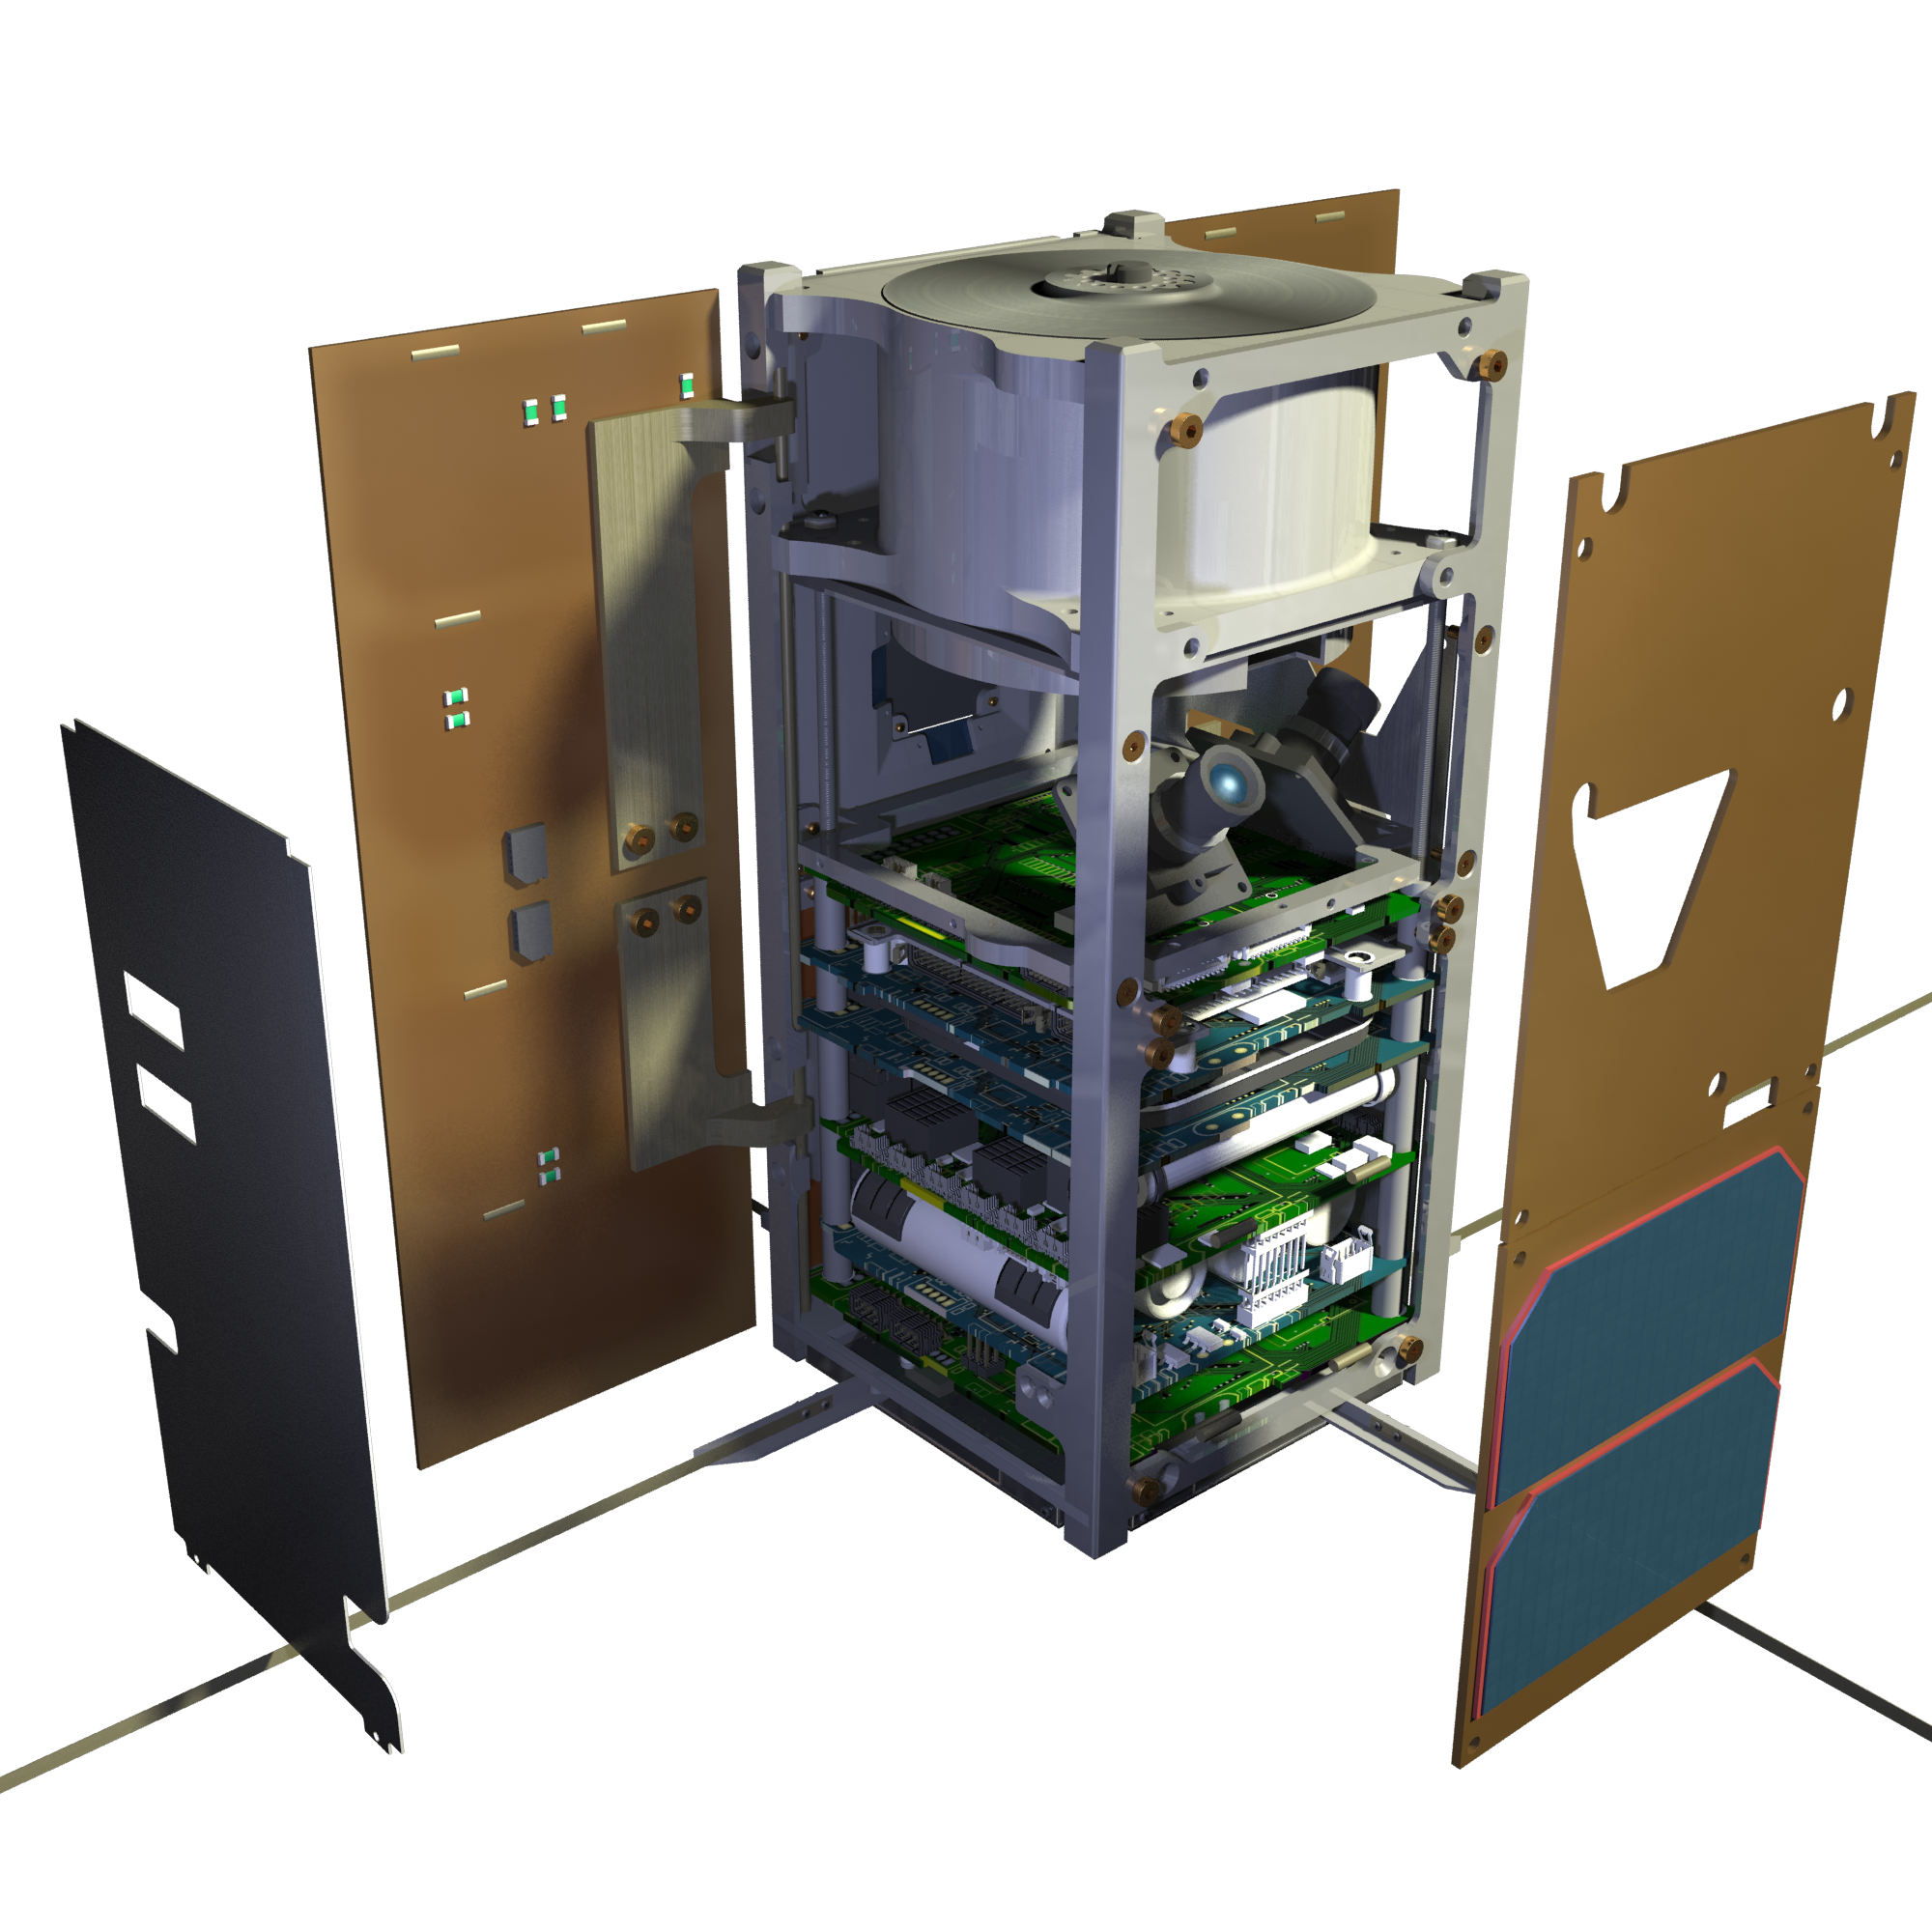
\includegraphics[width=0.5\paperwidth]{img/04/PW-Sat2_render_01.png}
        \caption{PW-Sat2 render (by M. Świetlik)}
        \label{PW-Sat_render_01}
    \end{figure}

    PW-Sat2 is scheduled to be launched on Falon9 rocket from SpaceX company in Q4 2017.

    \begin{figure}[H]
        \centering
           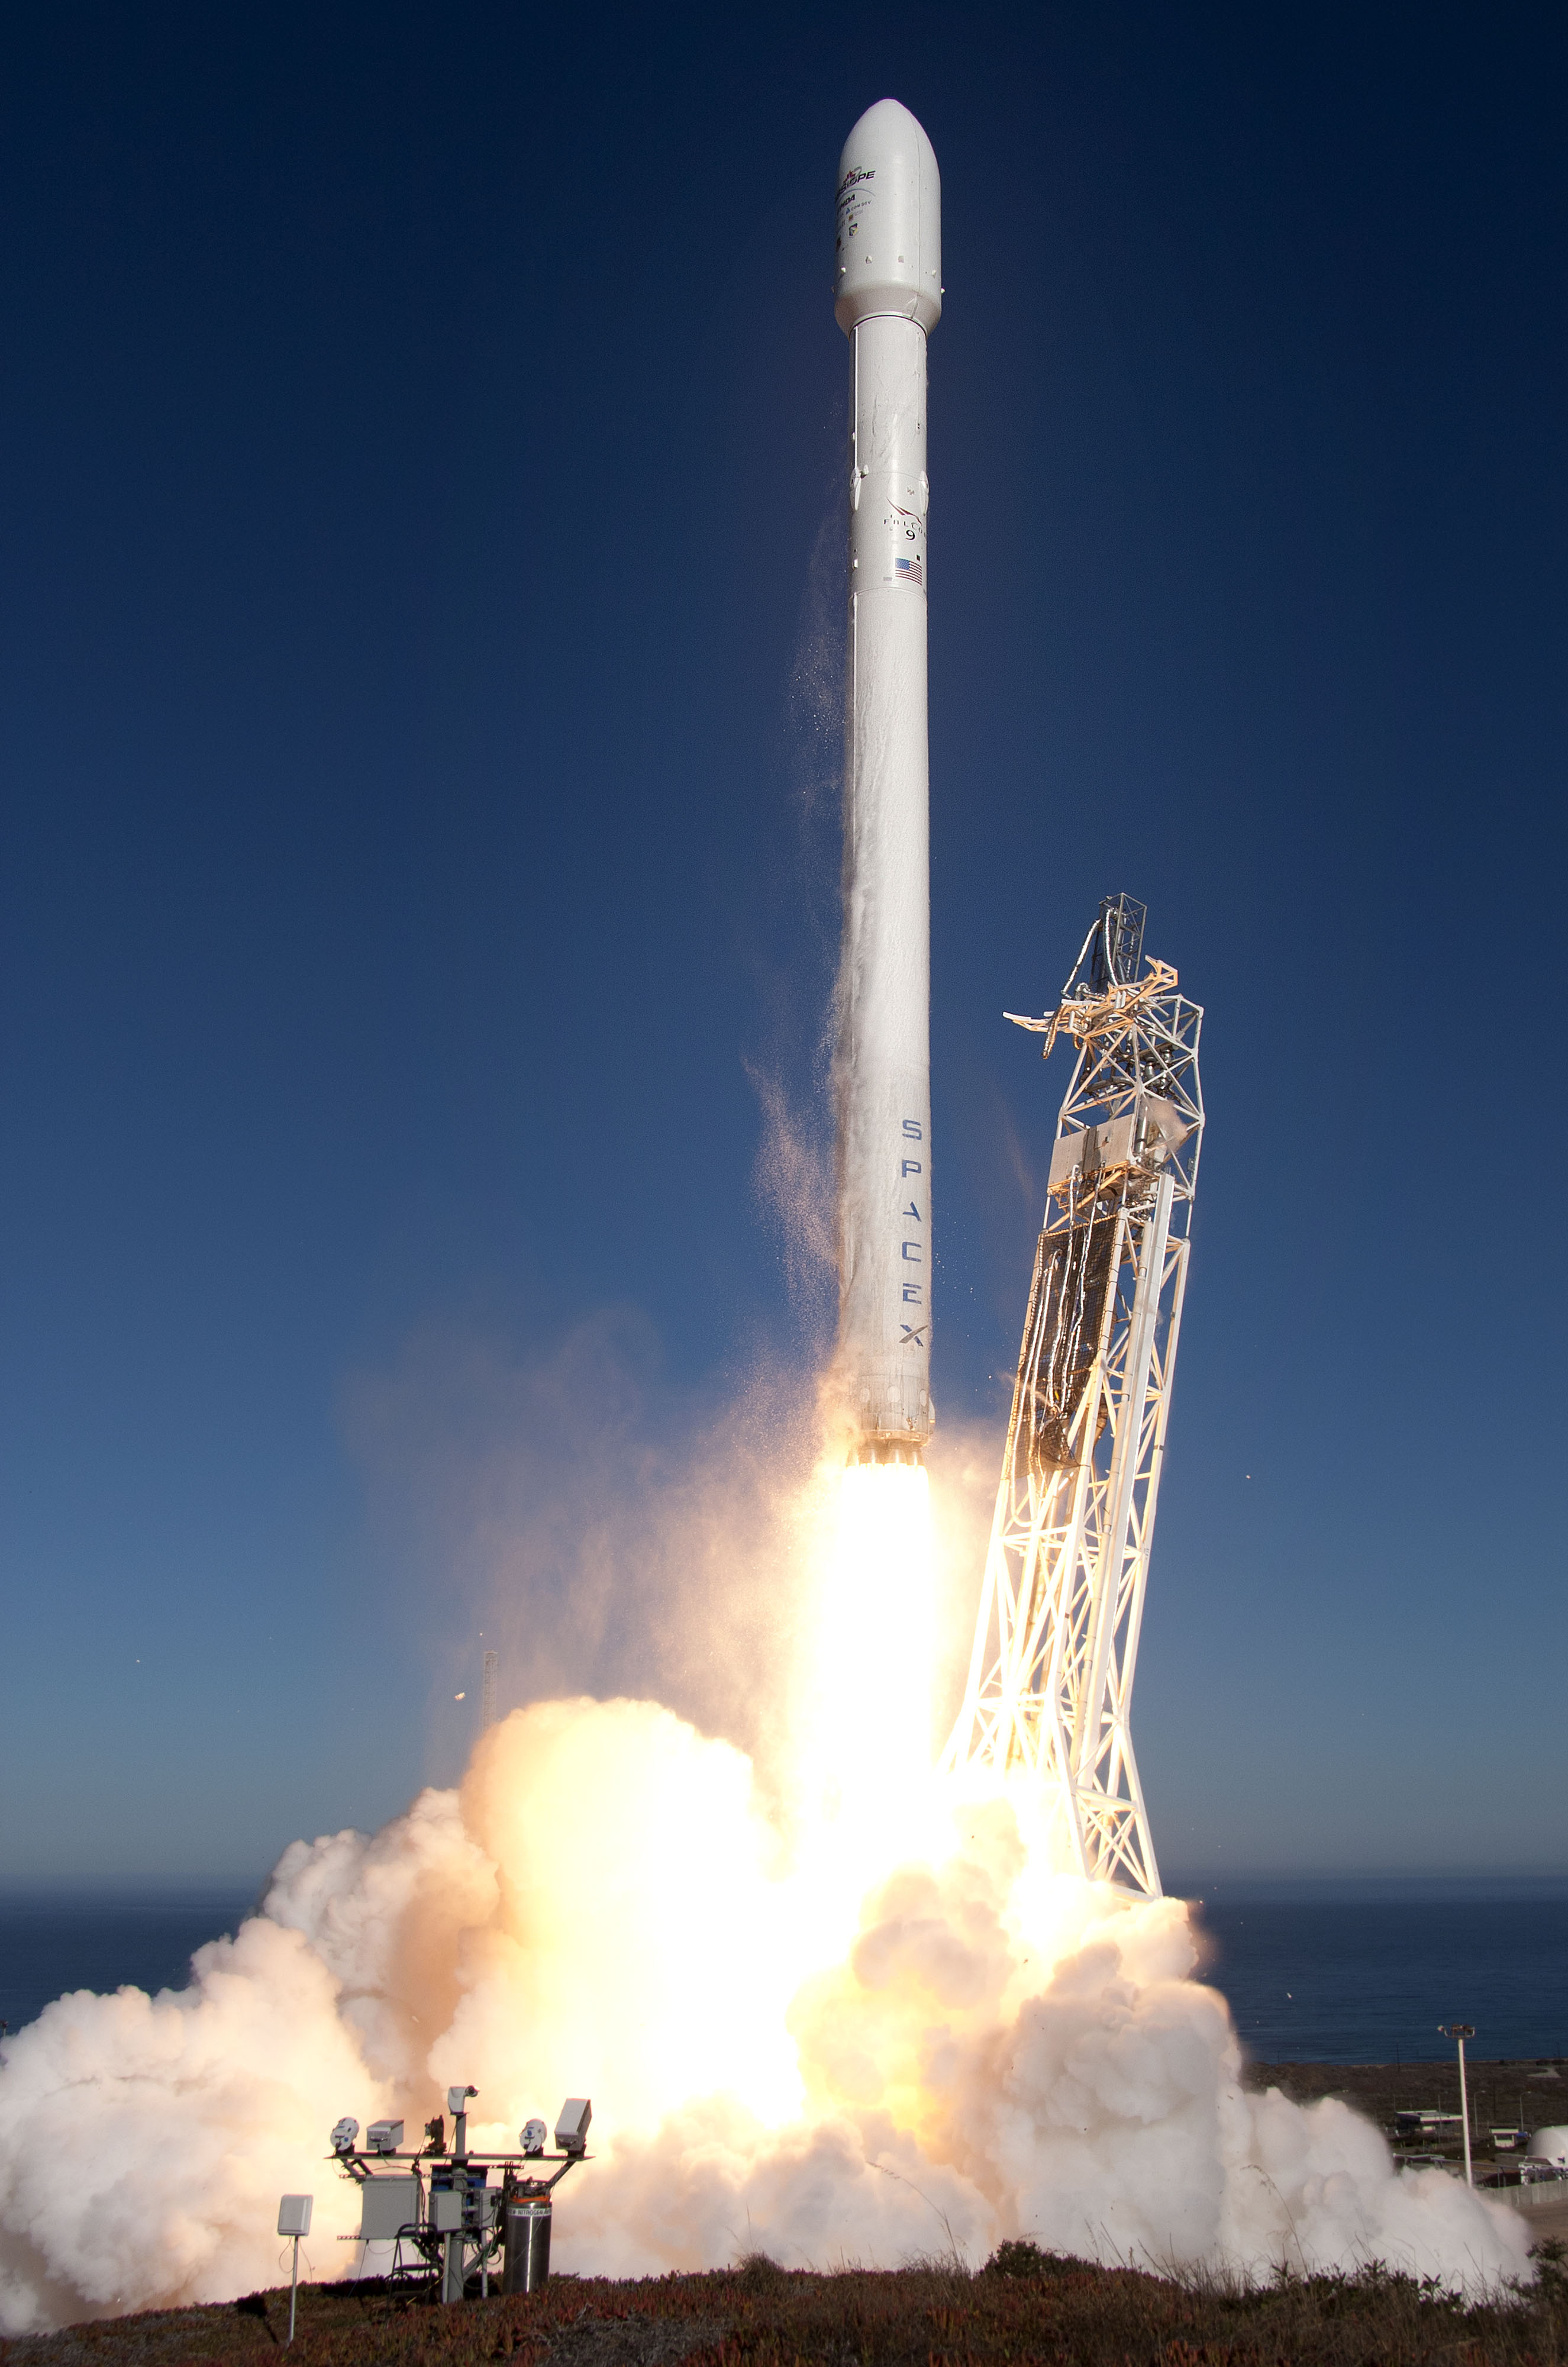
\includegraphics[width=0.3\paperwidth]{img/04/Falcon9.jpg}
        \caption{Falcon9 rocket. Source: \url{www.spacex.com}}
        \label{Falcon9}
    \end{figure}


    \subsection{Primary mission}
        Primary mission of PW-Sat2 is to test deorbit sail. Its purpose is to increase atmospheric drag and shorten satellite life. This method of deorbitation could be easy way to reduce space debris on LEO. Render of PW-Sat2 with opened sail is on \ref{PW-Sat_render_sail}.

        \begin{figure}[H]
            \centering
            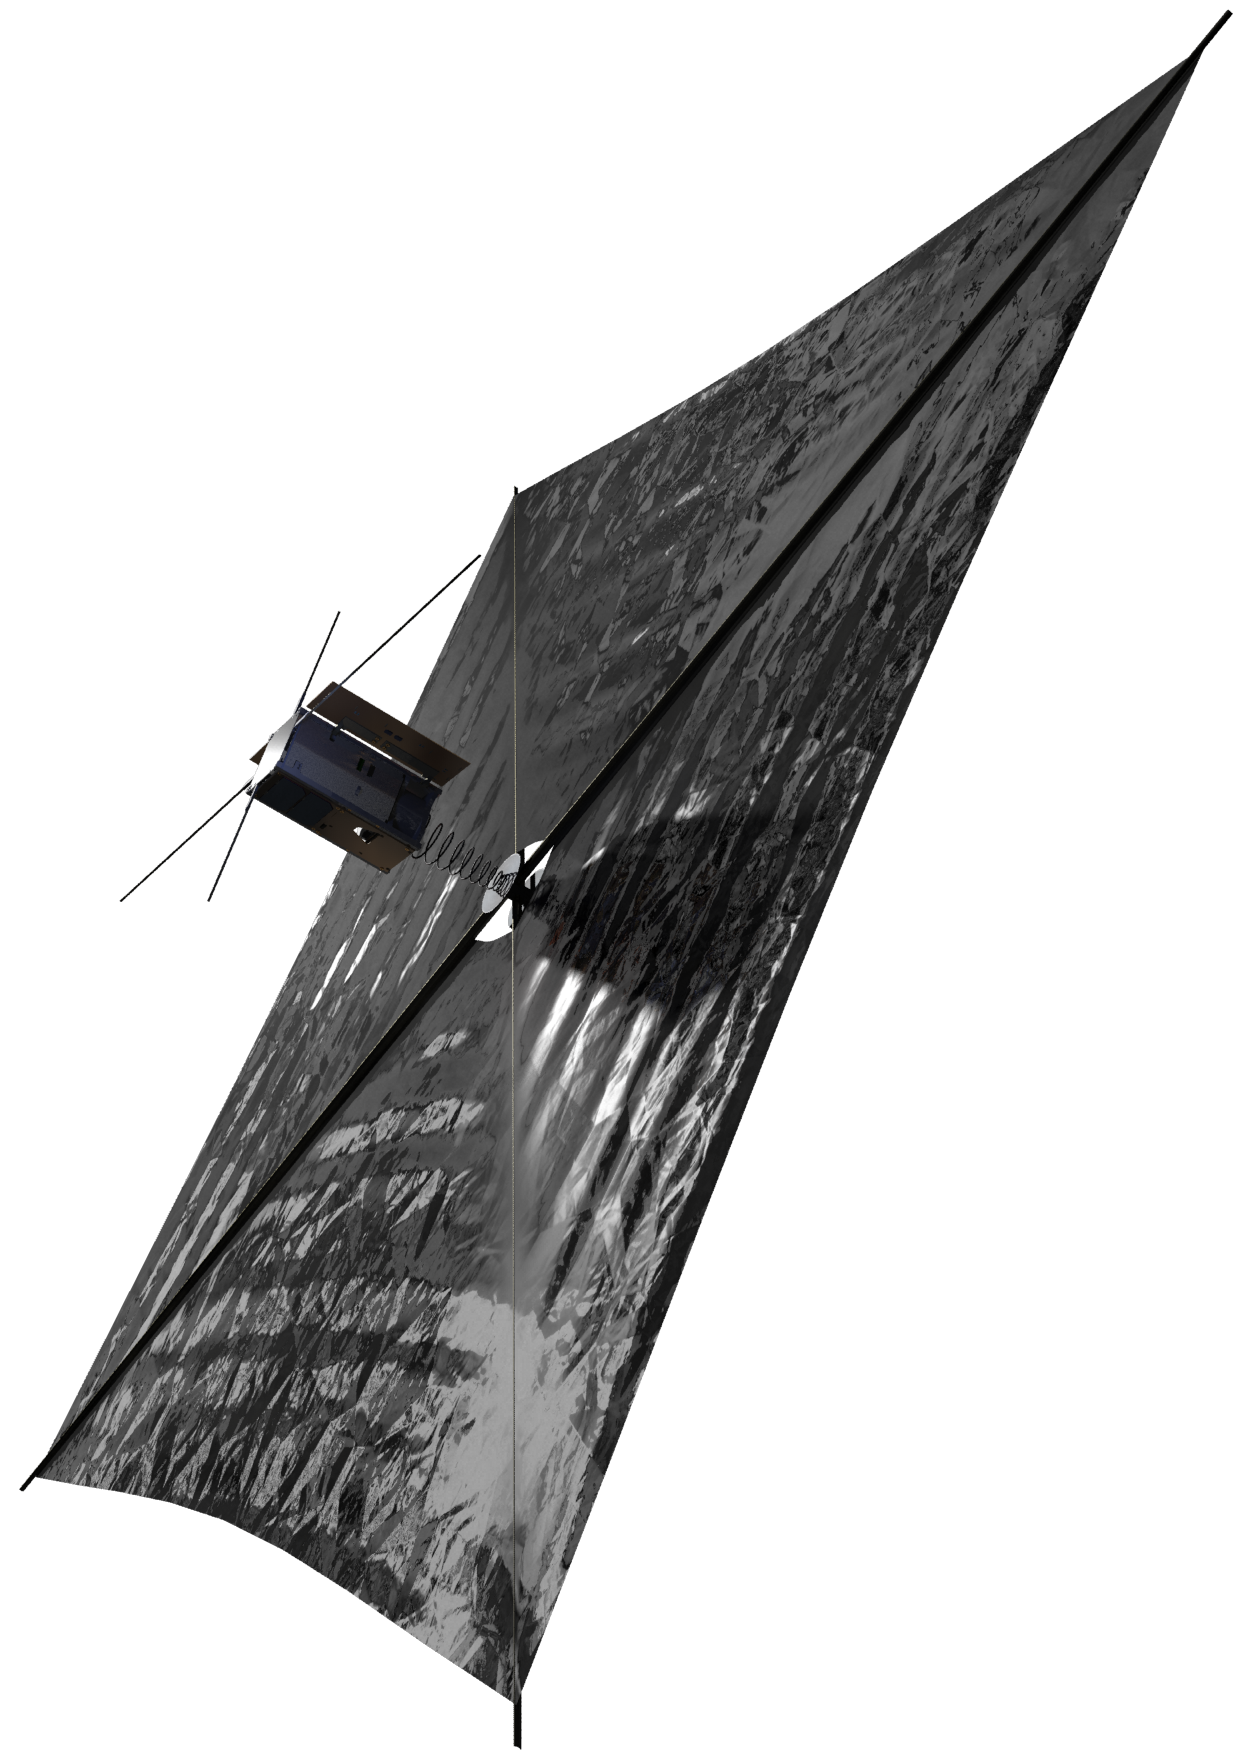
\includegraphics[width=0.7\paperwidth]{img/04/PW-Sat2_render_02.png}
            \caption{PW-Sat2 with opened sail (by M. Świetlik)}
            \label{PW-Sat_render_sail}
        \end{figure}

        More information about this experiment can be found in \cite{DDC_article}.

    \subsection{Lifetime}
        Due to its primary mission PW-Sat2 basic lifetime is planned to be 40 days long. After this time deorbit sail will open, and orbit will slowly decay. Deorbitation from nominal orbit is planned to take about one year \cite{PWSAT_MA_CDR}, but possibly with unreliable data connection. Therefore sensor should be able to measure dose absorbed during primary mission (40 days), but also to work during full predicted mission - about one year.

    \subsection{Orbit}
        PW-Sat2 in planned to be launched to sun-synchronous circular orbit of attitude \SI{575}{\kilo\meter}, with LTAN of 10:30 \cite{PWSAT_MA_CDR}.


    \subsection{Radiation analysis}
        Simulations in SPENVIS \cite{SPENVIS_URL} were performed to estimate TID accumulated during PW-Sat2 mission. On fig \ref{TIDvsSheilding} dose as a function of shielding thickness was plotted.

        \begin{figure}[H]
            \centering
            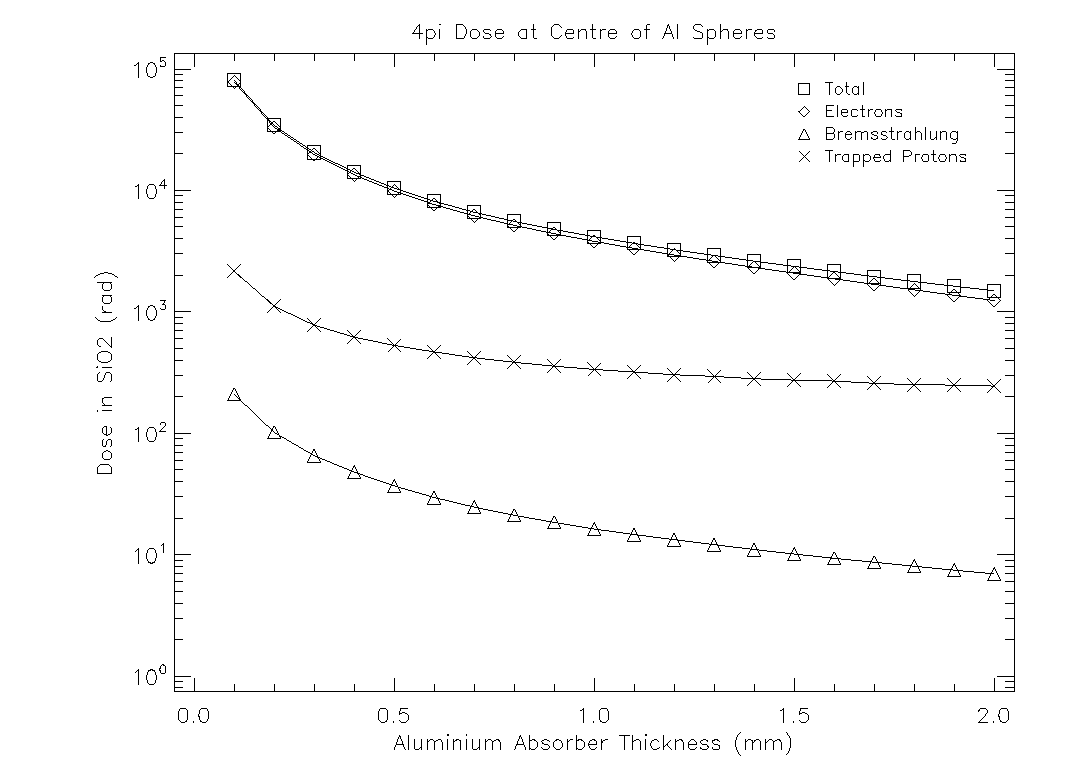
\includegraphics[width=0.7\paperwidth]{img/04/dose.eps}
            \caption{TID vs shielding}
            \label{TIDvsSheilding}
        \end{figure}

        Shielding of PW-Sat2 is about \SI{0.5}{\milli\meter} thick (aluminum sides as well as aluminum substrate for solar cells - \ref{PW-Sat_render_01}). Therefore  predicted dose during primary mission is \SI{1}{\kilo\rad} and during full mission about \SI{10}{\kilo\rad}.

\section{Sensor requirements}
    Summing PW-Sat2 mission analysis, high-level sensor requirements were estimated, summarized in table \ref{sensor_requirements_table}.

    \begin{table}[H]
        \begin{center}
            \begin{tabular}{r|l}
                \textbf{Requirement} & \textbf{Value} \\ \hline
                Range & \SI{10}{\kilo\rad} \\
                Resolution & \SI{10}{\rad} \\
                Total accuracy & \SI{\pm 100}{\rad}
            \end{tabular}
        \end{center}
        \caption{Sensor requirements}
        \label{sensor_requirements_table}
    \end{table}

\section{Applicable standards}
    The sensor should comply to ECSS \cite{ECSS_URL} standards. They are required by launch provider, and they describe good practices during space product development.

    ESCIES \cite{ESCIES_URL} provide valuable knowledge about components qualifications, testing and verification.

\section{Electrical requirements}
    Sensor will be placed on-board of PW-Sat2. Therefore it should comply to its' standards - power supplies, communication interfaces etc.

    \subsection{Electronics stack}
        Modules on PW-Sat2 are connected in PC-104 stack structure as shown in the figure \ref{PW-Sat2_stack}. Is is placed inside structure and consists of (from the top):
        \begin{itemize}
            \item \textbf{Payload module (PLD)} - where the sensor will be located,
            \item On-Board Computer (OBC) - main data processing unit,
            \item Attitude Determination and Control Subsystem (ADCS) - controls attitude (detumbling and sunpointing),
            \item Electrical Power System (EPS) - charges and discharges batteries, provides safety mechanisms,
            \item Battery module (ACC) - main energy storage,
            \item Communication transceiver (COMM) - VHF \& UHF full duplex transceiver,
            \item Antennas module (ANT) - antennas for uplink and downlink.
        \end{itemize}

        \begin{figure}[H]
            \centering
            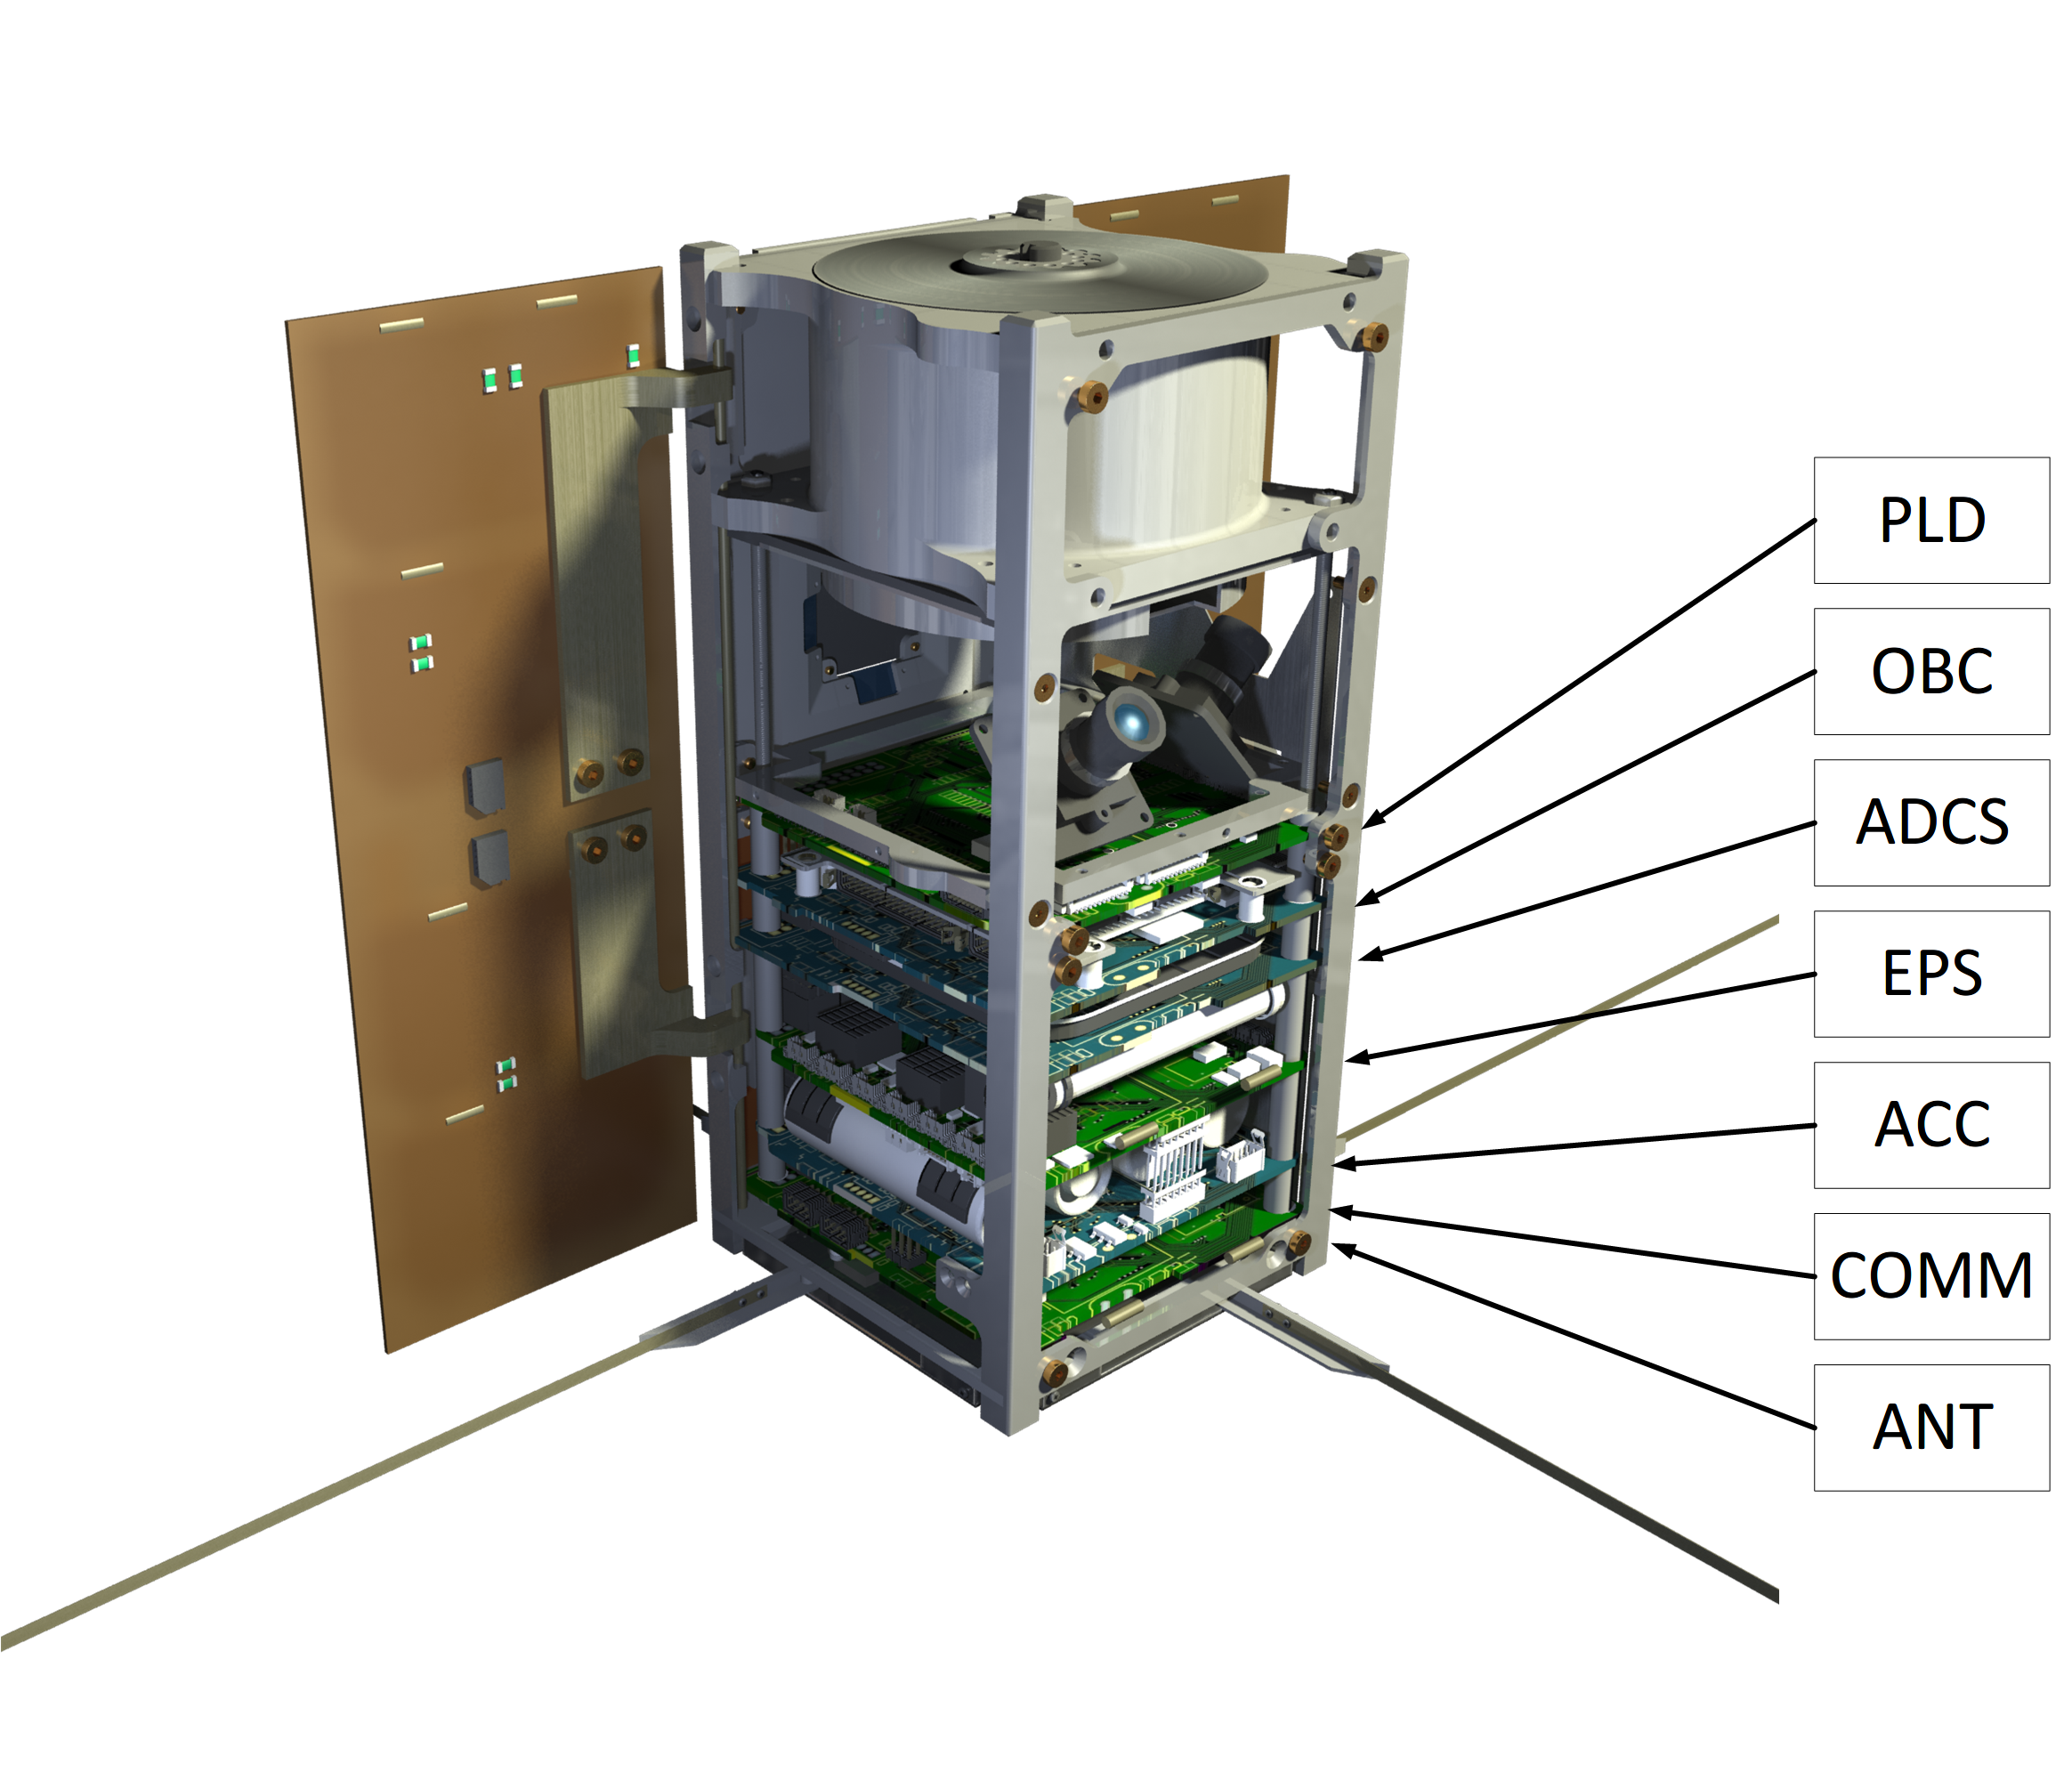
\includegraphics[width=0.7\paperwidth]{img/04/PW-Sat2-stack.png}
            \caption{PW-Sat2 electronics stack}
            \label{PW-Sat2_stack}
        \end{figure}

    \subsection{PC-104 connector}
        PLD board is connected to OBC with PC-104 connector. This connector provides data and power connections to satellite bus.

        This connector consists of:
        \begin{itemize}
            \item $I^2C$ bus, connected directly to MCU on OBC,
            \item interrupt line on which the sensor can notify OBC about command completion,
            \item SENS \SI{5}{\volt} line, powered only when sensor is commanded to be enabled.
        \end{itemize}

    \subsection{Power rail}
        As mentioned earlier, the power for the sensor is +\SI{5}{\volt}, activated whenever sensor should be accessed by OBC.

        Power line is controlled and protected by Latchup-Current Limiter FPF2701MX placed on EPS board. Therefore additional latchup protection in not necessary in this design. However, this sensor will be not only one on PLD board and should have it's own power switch. PLD board is enabled and disabled by EPS on OBC command and sensor should be enabled only during TID readout. Having this in mind forces the design to be immune to immediate shutdowns and dose have to be accumulated off-line.

    \subsection{Power consumption}
        During irradiation sensor should be completely turned off. It decreases possibility of radiation damage and increases overall system reliability.

        During readout required power should be less than \SI{1}{W}.

    \subsection{Data interface}
        The sensor is connected to OBC via $I^2C$ interface. OBC on this bus is master - and sensor should be one of slaves. PLD board can be disabled, therefore it should provide isolation of $I^2C$ bus when it is powered off.

    \subsection{Radiation immunity}
        Design should be itself immune to radiation. For PW-Sat2 threshold of \SI{10}{\kilo\rad} was chosen for all COTS components. Semiconductors should have radiation tests as described in \cite{ESCIES_TID_test_method}.

    \subsection{Electromagnetic compatibility}
        EMC requirements are described in \cite{ECSS_E_ST_20_07C}. This standard was tailored to PW-Sat2 because power rail is \SI{+5}{\volt}, other than on bigger spacecrafts (\SI{+28}{\volt}).

        \begin{itemize}
            \item Conducted susceptibility is shown in the figure \ref{EMC_conducted_susceptibility} . It was created by down-scaling figure A-4 from \cite{ECSS_E_ST_20_07C} by factor of $\SI{28}{\volt}/\SI{5}{\volt} = 5.6$. EMC limit on power line is defined as constant \SI{175}{\milli\volt} from \SI{30}{\hertz} to \SI{100}{\kilo\hertz}. Sensor should be able to filter this ripple to produce stable power for analog devices. In addition, it should be taken into account that output DC-DC converters on EPS runs on \SI{500}{\kilo\hertz}.

            \begin{figure}[H]
                \centering
                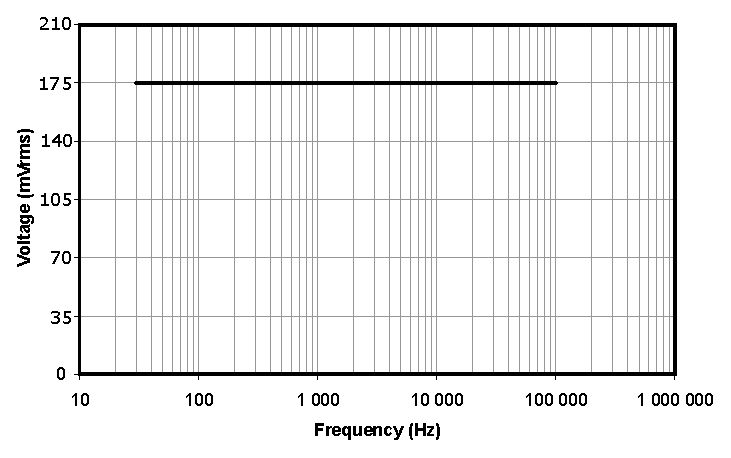
\includegraphics[width=0.5\paperwidth]{img/04/EMC_conducted_susceptibility.eps}
                \caption{Conducted susceptibility limit, frequency domain. Source: \cite{ECSS_E_ST_20_07C}}
                \label{EMC_conducted_susceptibility}
            \end{figure}


            \item Conducted emission is defined in the figure \ref{EMC_conducted_emission}.

            \begin{figure}[H]
                \centering
                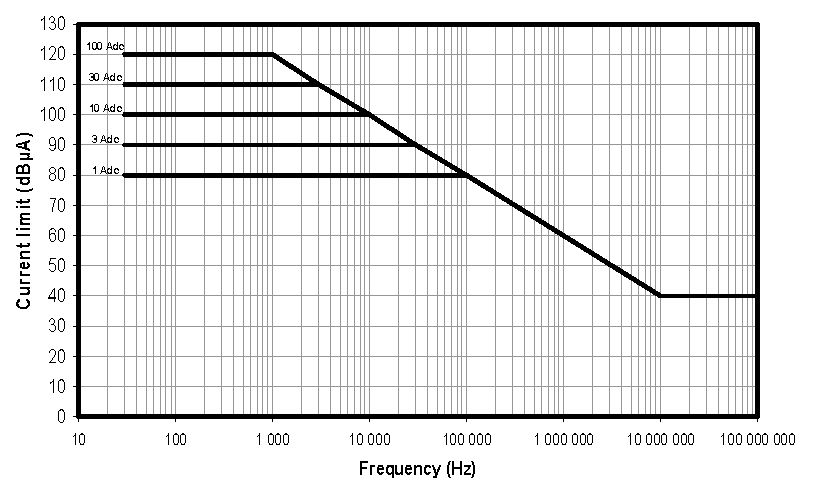
\includegraphics[width=0.5\paperwidth]{img/04/EMC_conducted_emission.eps}
                \caption{Conducted susceptibility limit, frequency domain. Source: \cite{ECSS_E_ST_20_07C}}
                \label{EMC_conducted_emission}
            \end{figure}


            \item Radiated susceptibility.
                On board PW-Sat2 is a communication module transmitting \SI{0.5}{\watt} of power on frequency \SI{435.02}{\mega\hertz}. It is planned that during readout radio transmitter will be disabled, but proper tests should be conducted to check for possible errors and faults.

                PLD board is placed near OBC - so radiated emission from digital lines can couple to sensor elements causing noise and errors. Proper tests will be conducted and if necessary shielding will be implemented.

            \item Radiated emission.
                Sensor is not predicted to emit any kind of radio waves. In case of detected anomaly further design decisions would have to be made.

        \end{itemize}


    \subsection{Inrush current}
        Inrush current have to be limited to maximum power consumption to not trigger LCL on EPS.

    \subsection{Reliability of components}
        This sensor is not a critical part of the satellite. But, reliable components should be used to ensure proper results.

        Every used component should have failure rate of $0.1\si{\percent}$ or lower. This is essential in capacitors and other passive components.


\section{Mechanical requirements}
    In this chapter design constrains and mechanical requirements of Falcon9 are presented. Launcher requirements were taken from \cite{Falcon9_user_manual}.

    \subsection{PCB}
    \label{PCB_description}
        PCB of PLD board is standard 4-layer FR4 board with stack shown in the figure \ref{PLD_PCB_stack}. Its dimensions are shown on \ref{PLD_PCB_size}, but design is forced to take much less space. For this sensor limits are \SI{3x3}{\centi\meter} double sided.

        \begin{figure}[H]
            \centering
            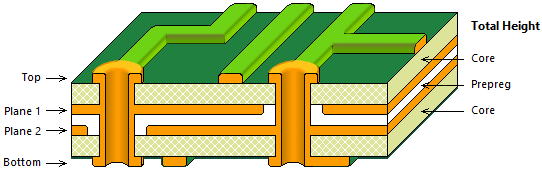
\includegraphics[width=0.5\paperwidth]{img/04/PLD_PCB_stack.png}
            \caption{PLD board PCB stack}
            \label{PLD_PCB_stack}
        \end{figure}

        \begin{figure}[H]
            \centering
            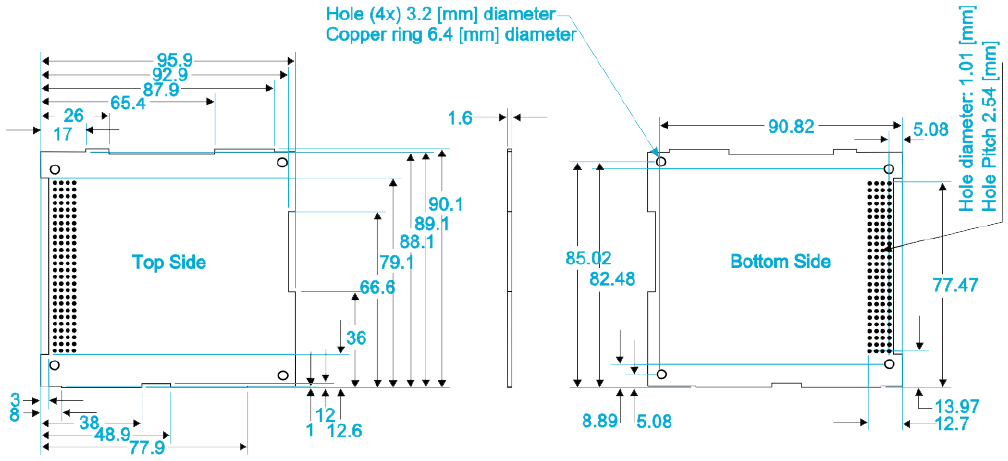
\includegraphics[width=0.7\paperwidth]{img/04/PC104_PLD_size.png}
            \caption{PC-104 size}
            \label{PLD_PCB_size}
        \end{figure}



    \subsection{Outgassing}
        Every used component should be able to work in vacuum. Outgassing of components should be known to conduct required vacuum tests before launch. Too big outgassing coefficient can result in damage of turbomolecular pump in vacuum chamber.

    \subsection{Vibration}
        During rocket launch large vibrations occur on payload, therefore it should be immune to it. In case of any heavy electronic components appropriate glue should be applied to prevent joint cracks.
        \begin{figure}[H]
            \centering
            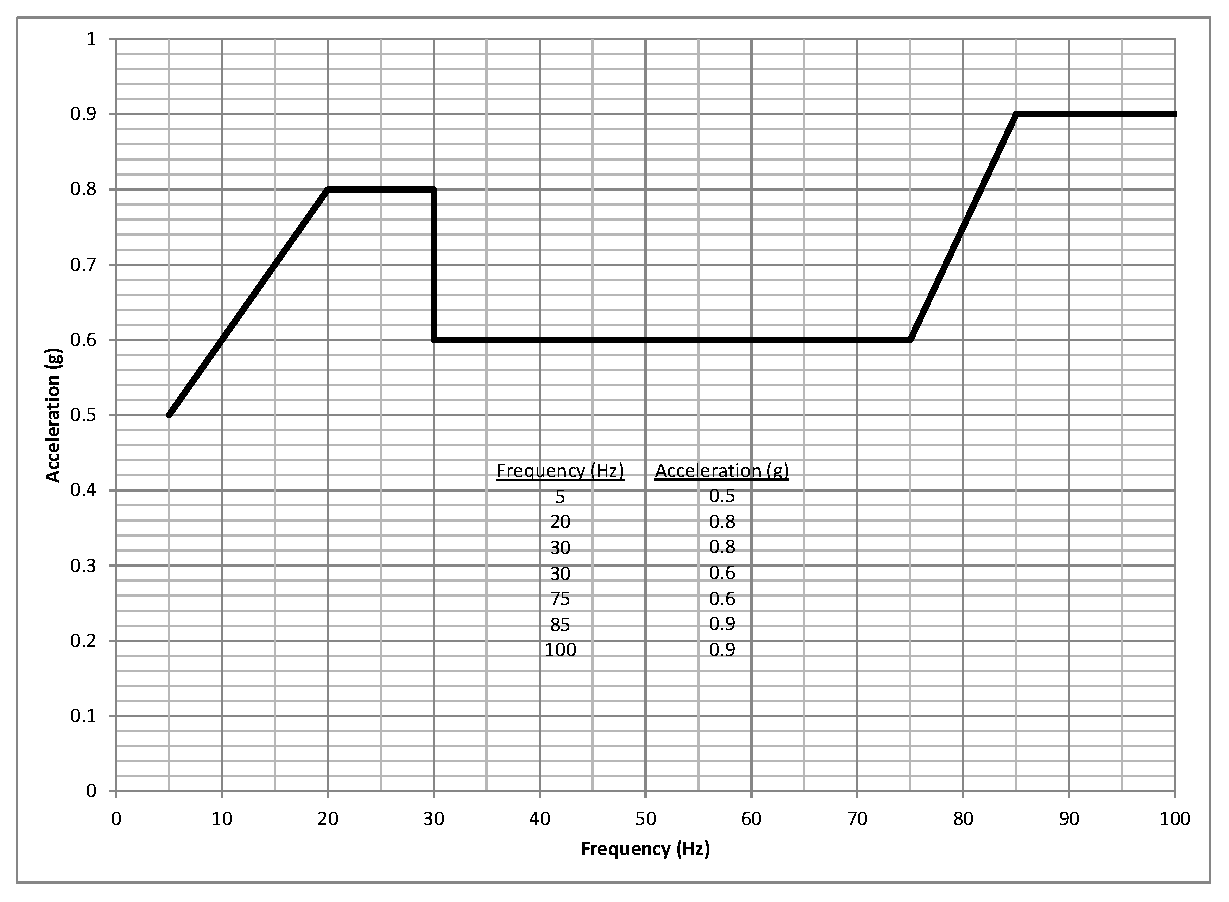
\includegraphics[width=0.5\paperwidth]{img/04/Falcon9_vibration.eps}
            \caption{Falcon9 maximum axial equivalent sine environment. Source: \cite{Falcon9_user_manual}}
            \label{Falcon9_vibration}
        \end{figure}


    \subsection{Operation temperature}
        The sensor should work in every operational case satellite can be. Simulations were performed to find bounds of possible temperature range inside satellite.    In \cite{PWSAT_TCS_CDR} results are presented.

        For PLD board operation range is $\SI{0}{\degreeCelsius}$ to $\SI{60}{\degreeCelsius}$. If the measured temperature will be outside this region, sensor will not be enabled.


    \subsection{Thermal cycles}
        Or PW-Sat2 orbit sun illumination is changing every $\approx \SI{90}{\minute}$. Therefore large number of thermal cycles are applied to On-Board electronics, which can cause joint cracks as well as component failures. Proper soldering and component selection will be made, according to ECSS.

        As described in \cite{ECSS_Q_ST_70_04C} the sensor should pass thermal cycle tests: $100$ times from $- (100 \pm 5)$\si{\degreeCelsius} to $(100 \pm 5)$\si{\degreeCelsius} in vacuum environment. Test procedure is shown on \ref{thermal_tests}.

        \begin{figure}[H]
            \centering
            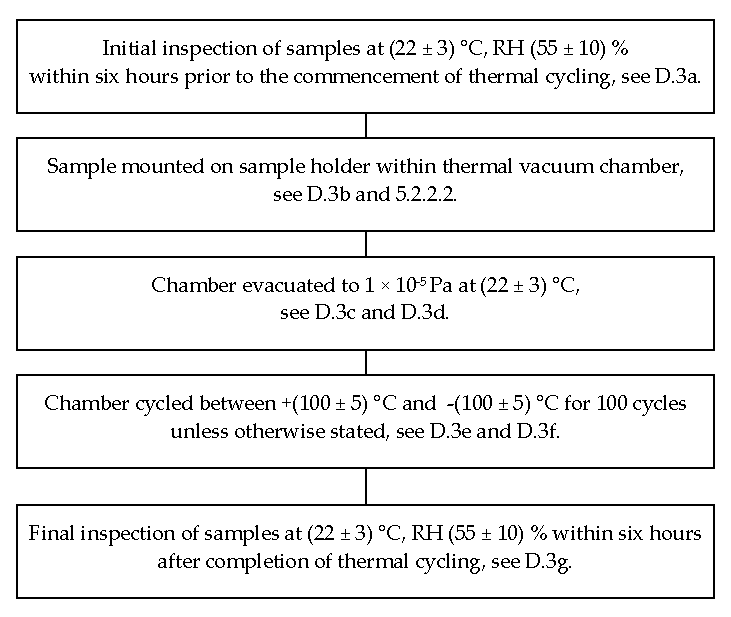
\includegraphics[width=0.5\paperwidth]{img/04/thermal_cycles.eps}
            \caption{Thermal cycles test procedure. Source: \cite{ECSS_Q_ST_70_04C}}
            \label{thermal_tests}
        \end{figure}
